\section{Implementation}


\subsection{Reuse optimization}
The current \gls{mhc} method requires six lines of the image to be available in local memory for efficient operation.
Techincally it woulb be possible to use only five, but this would result in more cumb

\subsection{Efficient Separation}
The \gls{volta} has 48KiB of available shared memory per block \cite{rigerunNVIDIAJetsonXavier2023}.
With an image width of 2448 pixels \cite{lucidvisionlabsTriton0MPPolarization} it is only possible to store 10 lines in local shared memory.
\begin{align}
    \frac{48Kib}{2448px/line * 16b/px} = \frac{393216b}{39168b/l} \approx 10.039line
\end{align}
Not problem on Orin.


\begin{figure}[H]
    \centering
    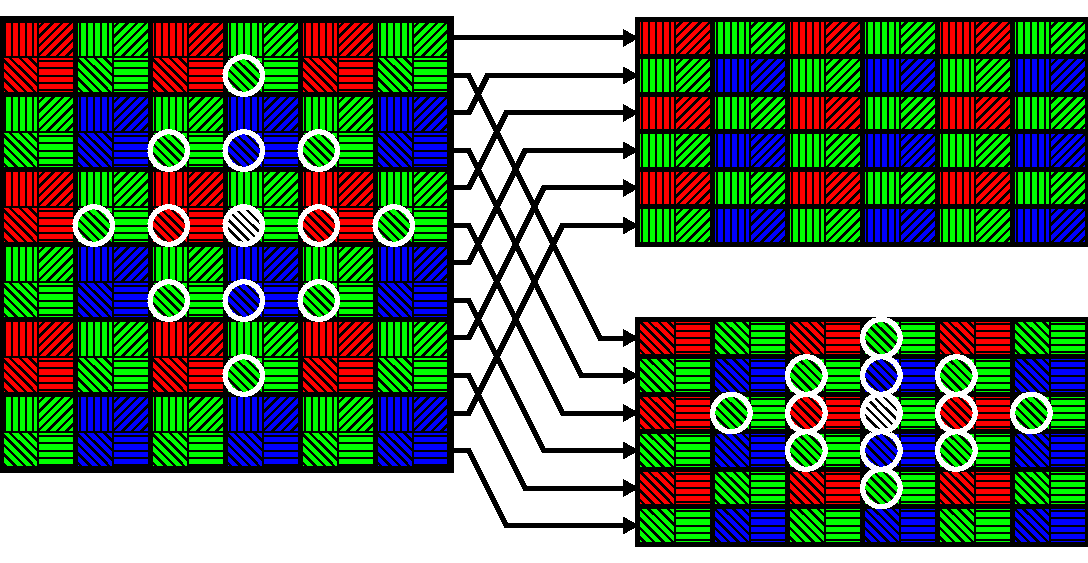
\includegraphics[width=\textwidth]{figures/polarized_image/separation.pdf}
\end{figure}

\begin{figure}[H]
    \centering
    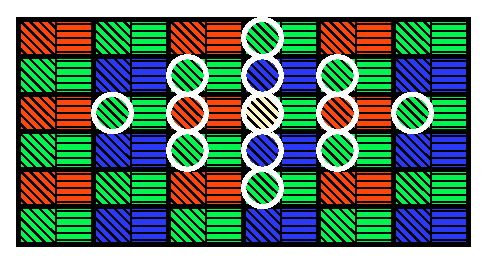
\includegraphics[width=.6\textwidth]{figures/polarized_image/separated_conv.pdf}
\end{figure}




With a runtime of $1 ms \pm 1 \mu s$
Nsight compute not working for memory







\subsubsection{Use of constant memory}
During the development process it was tested whether storing the constant values used in the debayer algorithm in constant memory would speed up the process.
Constant memory is a type of limited read-only memory available on NVIDIA \glsps{gpu} \cite[61]{nvidiaCUDABestPractices2023}.
NVIDIA \glspl{gpu} only have 64KiB of constant memory \cite[61]{nvidiaCUDABestPractices2023}.
Read instruction from constant memory are very efficient and the best performance is acheived when all threads in a warp, as opposed to regular memory where this would result in inefficient collisions \cite[61]{nvidiaCUDABestPractices2023} \cite[13,14]{volkovLatencyHiding2016}
As the different threads in each warp would need the same constants this is ideal.

All unique constant variables used in the algorithm were collected as a part of the automatic code generation and stored in a constant device array.
Unfortynately this change had no visible impact on the performance.
A minimal test was later created that performed a very simple repeated multiply and add operation, where the coefficient and constats were either stored in constant memory or defined expicitly in the funciton as shown in \code{mfa_1} and \code{mfa_2} in Listing \ref{listing:cuda_mem_tests}.
This minimal tests showed that using constant memory was actually marginally slower (0.08\% on average) than using explicit values.

Further it was tested weither the compiled code would beform better if the values in local constant variables as in the \code{mfa_3} function in Listing \ref{listing:cuda_mem_tests}.
This gave marginally better results than \code{mfa_1} (0.04\% on average), but was deemed unecessery to implement.

\begin{listing}[H]
    \begin{minted}{cuda}
        __device__ __forceinline__ __half2 mfa_1(__half2 a) {
        return __hfma2(__float2half2_rn(0.098f), a, __float2half2_rn(3.14f));
        }
        __device__ __forceinline__ __half2 mfa_2(__half2 a) {
            return __hfma2(constant_mem[0], a, constant_mem[1]);
        }
        __device__ __forceinline__ __half2 mfa_3(__half2 a) {
            const __half2 b = __float2half2_rn(0.098f);
            const __half2 c = __float2half2_rn(3.14f);
            return __hfma2(b, a, c);
        }
    \end{minted}
    \caption{Small functions used to test local memory implementations.}
    \label{listing:cuda_mem_tests}
\end{listing}



\subsection{Better reading}
Another improvement was to use an array of pointers, rather than an array of arrays.
Initially the the section of the image on which calculations were performed were stored as an array of arrays in local shared memory.
When the computations on that part was performed, the whole block would move down.
\begin{figure}[H]
    \centering
    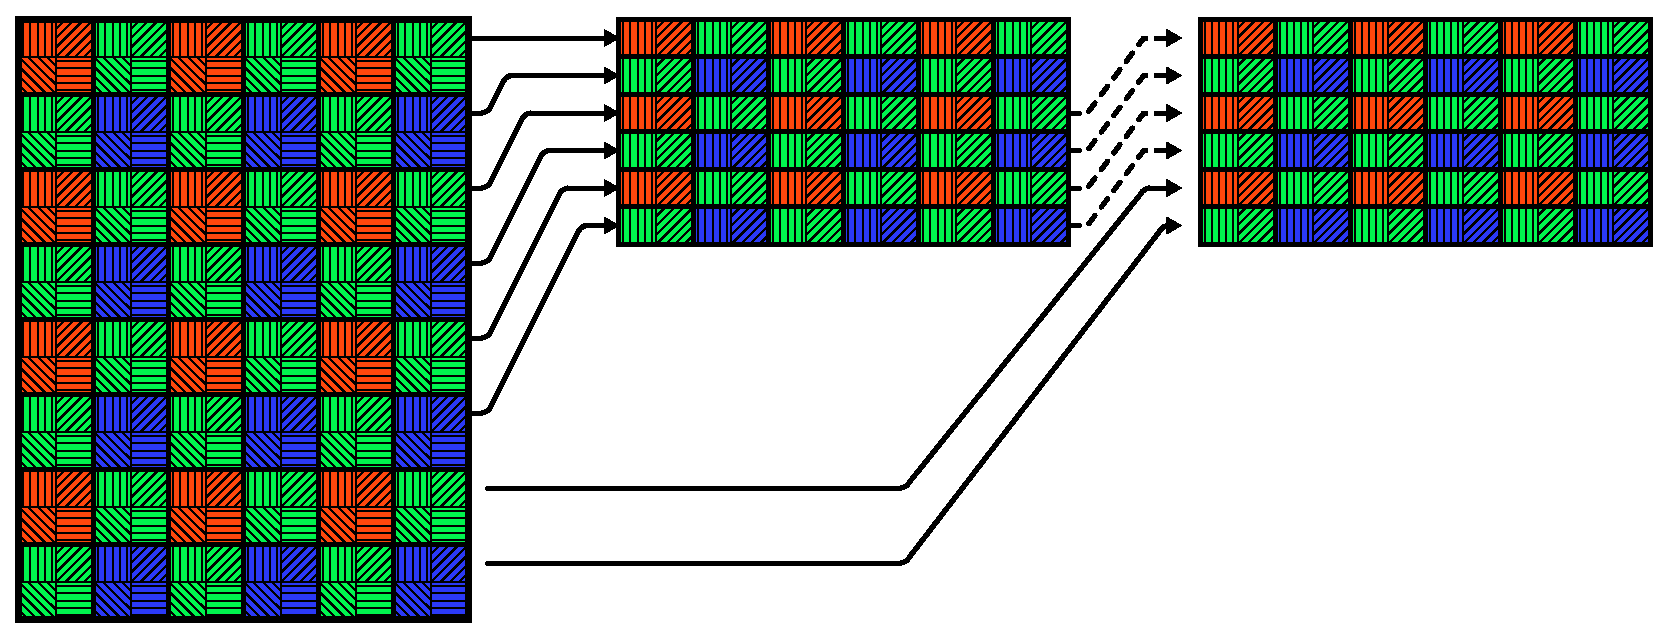
\includegraphics[width=\textwidth]{figures/polarized_image/read_line.pdf}
    \caption{TODO}
\end{figure}


\subsection{Half precitions floating point}